%________________________________________________________
\section{Analysis framework}
\label{Note:ANALYSIS}

Recently, a new attempt has started that led to the development of a a new analysis framework \cite{Note:RefAnalysisFramework}. By the time this note was being written the framework has been validated in processes that concern this document (GRID analysis). We will review the basic classes and functionalities of this system in this paragraph (for further details the reader should look in \cite{Note:RefAnalysisFramework,Note:RefAlienTutorial}).

The basic classes that form this development are the following (we will give a full example of an overall implementation later):

\begin{itemize}
\item {\ttfamily AliAnalysisDataContainer:} The class that allows the user to define the basic input and output containers.
\item {\ttfamily AliAnalysisTask:} This is the class the lines of which should be implemented by the user. In the source file we can write the analysis code. 
\item {\ttfamily AliAnalysisManager:} Inside such a manager the user defines the analysis containers, the relevant tasks as well as the connection between them.
\end{itemize}

A practical example of a simple usage of this framework is given below where we extract a $P_{T}$ spectrum of all charged tracks (histogram) from an ESD chain (the examples can be found under the AnalysisMacros/Local/ directory of the PWG2 module of AliRoot).

\vspace{0.5 cm}
\textbf{AliAnalysisTaskPt.h}
\begin{lstlisting}[language=C++]
  #include "TH1.h"
  #include "AliESD.h"
  #include "AliAnalysisTask.h"

  class AliAnalysisTaskPt : public AliAnalysisTask {
    public:
    AliAnalysisTaskPt(const char *name);
    virtual ~AliAnalysisTaskPt() {}
    
    virtual void   Init(Option_t *);
    virtual void   Exec(Option_t *option);
    virtual void   Terminate(Option_t *);
    
    private:
    AliESD *fESD; //ESD object
    TH1F   *fHistPt; //Pt spectrum
    
    ClassDef(AliAnalysisTaskPt, 0); // example of analysis
  };
\end{lstlisting}

\vspace{0.5 cm}
\textbf{AliAnalysisTaskPt.cxx}
\begin{lstlisting}[language=C++]
  #define AliAnalysisTaskPt_cxx

  #include "TChain.h"
  #include "TH1.h"
  #include "TCanvas.h"
  #include "TSystem.h"
  #include "AliAnalysisTask.h"
  #include "AliESD.h"
  
  #include "AliAnalysisTaskPt.h"
  
  ClassImp(AliAnalysisTaskPt)
  
  //________________________________________________________________________
  AliAnalysisTaskPt::AliAnalysisTaskPt(const char *name) 
  :AliAnalysisTask(name,""), fESD(0), fHistPt(0) {
    // Constructor.
    // Input slot #0 works with a TChain
    DefineInput(0, TChain::Class());
    // Output slot #0 writes into a TH1 container
    DefineOutput(0, TH1F::Class());
  }
  
  //________________________________________________________________________
  void AliAnalysisTaskPt::Init(Option_t *) {
    printf("   Init %s\n", GetName());
    
    if (!fESD) {
      char ** address = (char **)GetBranchAddress(0, "ESD");
      if (address) fESD = (AliESD*)(*address);
      if (!fESD) {
	fESD = new AliESD();
	SetBranchAddress(0, "ESD", &fESD);
      }
      OpenFile(0,"Pt.ESD.1.root","RECREATE");
    }
    
    if (!fHistPt) {
      fHistPt = new TH1F("fHistPt","This is the Pt distribution",15,0.1,3.1);
      fHistPt->SetStats(kTRUE);
      fHistPt->GetXaxis()->SetTitle("P_{T} [GeV]");
      fHistPt->GetYaxis()->SetTitle("#frac{dN}{dP_{T}}");
      fHistPt->GetXaxis()->SetTitleColor(1);
      fHistPt->SetMarkerStyle(kFullCircle);
    }
  }
  
  //________________________________________________________________________
  void AliAnalysisTaskPt::Exec(Option_t *) {
    // Task making a pt distribution.
    // Get input data
    TChain *chain = (TChain*)GetInputData(0);
    Long64_t ientry = chain->GetReadEntry();
    if (!fESD) return;
    
    printf("Tracks: %d \n",fESD->GetNumberOfTracks());
    for(Int_t iTracks = 0; iTracks < fESD->GetNumberOfTracks(); iTracks++) {
      AliESDtrack * ESDTrack = fESD->GetTrack(iTracks);
      Double_t momentum[3];
      ESDTrack->GetPxPyPz(momentum);
      Double_t Pt = sqrt(pow(momentum[0],2) + pow(momentum[1],2));
      fHistPt->Fill(Pt);
    }//track loop 
    // Post final data. It will be written to a file with option "RECREATE"
    PostData(0, fHistPt);
  }      
  
  //________________________________________________________________________
  void AliAnalysisTaskPt::Terminate(Option_t *) {
    // Draw some histogram at the end.
    if (!gROOT->IsBatch()) {
      TCanvas *c1 = new TCanvas("c1","Pt",10,10,310,310);
      c1->SetFillColor(10);
      c1->SetHighLightColor(10);   
      c1->cd(1)->SetLeftMargin(0.15);
      c1->cd(1)->SetBottomMargin(0.15);  
      c1->cd(1)->SetLogy();
      fHistPt->DrawCopy("E");
    }
  }
\end{lstlisting}

The {\ttfamily AliAnalysisTaskPt} is a sample task that inherits from the {\ttfamily AliAnalysisTask} class. The main functions that need to be implemented are the following:

\begin{itemize}
\item Basic constructor: Inside the constructor we need to define the type of the input (if any input is to be used) as well as of the output of the task (in our example the input is of the form of a ROOT's {\ttfamily TChain} while the output is a histogram - {\ttfamily TH1F}).
\item {\ttfamily Init:} Inside this function we need to initialize the objects, assign the branch addresses to these objects, create the output file as well as the output histograms (as in our example) or objects.
\item {\ttfamily Exec:} The place where the analysis code should be implemented.
\item {\ttfamily Terminate:} The function inside of which we can draw histograms (as in our example) or perform any kind of actions (like merging of output).
\end{itemize}

\vspace{0.5 cm}
\textbf{Macro that creates an AliAnalysisManager}
\begin{lstlisting}[language=C++]
  //____________________________________________//
  // Make the analysis manager
  AliAnalysisManager *mgr = new AliAnalysisManager();
  //____________________________________________//
  // 1st Pt task
  AliAnalysisTask *task1 = new AliAnalysisTaskPt("TaskPt");
  mgr->AddTask(task1);
  // Create containers for input/output
  AliAnalysisDataContainer *cinput1 = mgr->CreateContainer("cchain1",
  TChain::Class(),AliAnalysisManager::kInputContainer);
  AliAnalysisDataContainer *coutput1 = mgr->CreateContainer("chist1", 
  TH1::Class(),AliAnalysisManager::kOutputContainer);
  
  //____________________________________________//
  mgr->ConnectInput(task1,0,cinput1);
  mgr->ConnectOutput(task1,0,coutput1);
  cinput1->SetData(chain1);
  
  if (mgr->InitAnalysis()) {
    mgr->PrintStatus();
    chain1->Process(mgr);
  }
\end{lstlisting}

\vspace{0.2 cm}
In the previous lines we firstly created a new analysis manager:\\
\\
{\ttfamily AliAnalysisManager *mgr = new AliAnalysisManager();}\\
\\
We then created a new {\ttfamily AliAnalysisTaskPt} object giving it a name and we assigned it to the manager:\\
\\
{\ttfamily AliAnalysisTask *task1 = new AliAnalysisTaskPt("TaskPt");}\\
{\ttfamily mgr->AddTask(task1);}\\
\\
Then the input and output containers were created while defining in parallel their types: \\
\\
{\ttfamily AliAnalysisDataContainer *cinput1 = mgr->CreateContainer("cchain1", TChain::Class(),AliAnalysisManager::kInputContainer);}\\
{\ttfamily AliAnalysisDataContainer *coutput1 = mgr->CreateContainer("chist1", TH1::Class(),AliAnalysisManager::kOutputContainer);}\\
\\
The next step was to link the task with the corresponding input and output container while setting the created chain of files (in the following section we will review how we can create this chain) to our input:\\
\\
{\ttfamily mgr->ConnectInput(task1,0,cinput1);}\\
{\ttfamily mgr->ConnectOutput(task1,0,coutput1);}\\
{\ttfamily cinput1->SetData(chain1);}\\
\\
Finally we process the chain with the manager:\\
\\
{\ttfamily   if (mgr->InitAnalysis()) chain1->Process(mgr);}\\

\vspace{0.5 cm}
In order for the user to have an idea of how the framework could look like in a complicated example, we provide figures \ref{Note:FigAnalysisFramework1} and \ref{Note:FigAnalysisFramework2}. In fig. \ref{Note:FigAnalysisFramework1} we show the flow of a typical analysis process:

A user interacts with the file catalog and creates a tag collection (the reader should check section \ref{Note:FLOW} for the instructions on how to perform this action). Then the \tag is queried (details on how we can do this will be provided in the next sections) and a chain of files is created. While looping the entries of this chain we split our analysis into two branches, on the first of which we analyze the (real or simulated) data and we provide as a last step an output ROOT file with histograms, while on the second we mix the events (event mixing method) in order to express our background. This second branch creates an output of the form of an Analysis Object Data (AOD) \cite{Note:RefComputingTDR}. A new chain is then created from this AOD and after analyzing the corresponding entries (analysis of mixed events) the output ROOT file with the relevant histograms is created. Finally, a last process is launched that compares the two output ROOT files and extracts the studied signal.


\begin{figure}[ht!]
\begin{center}
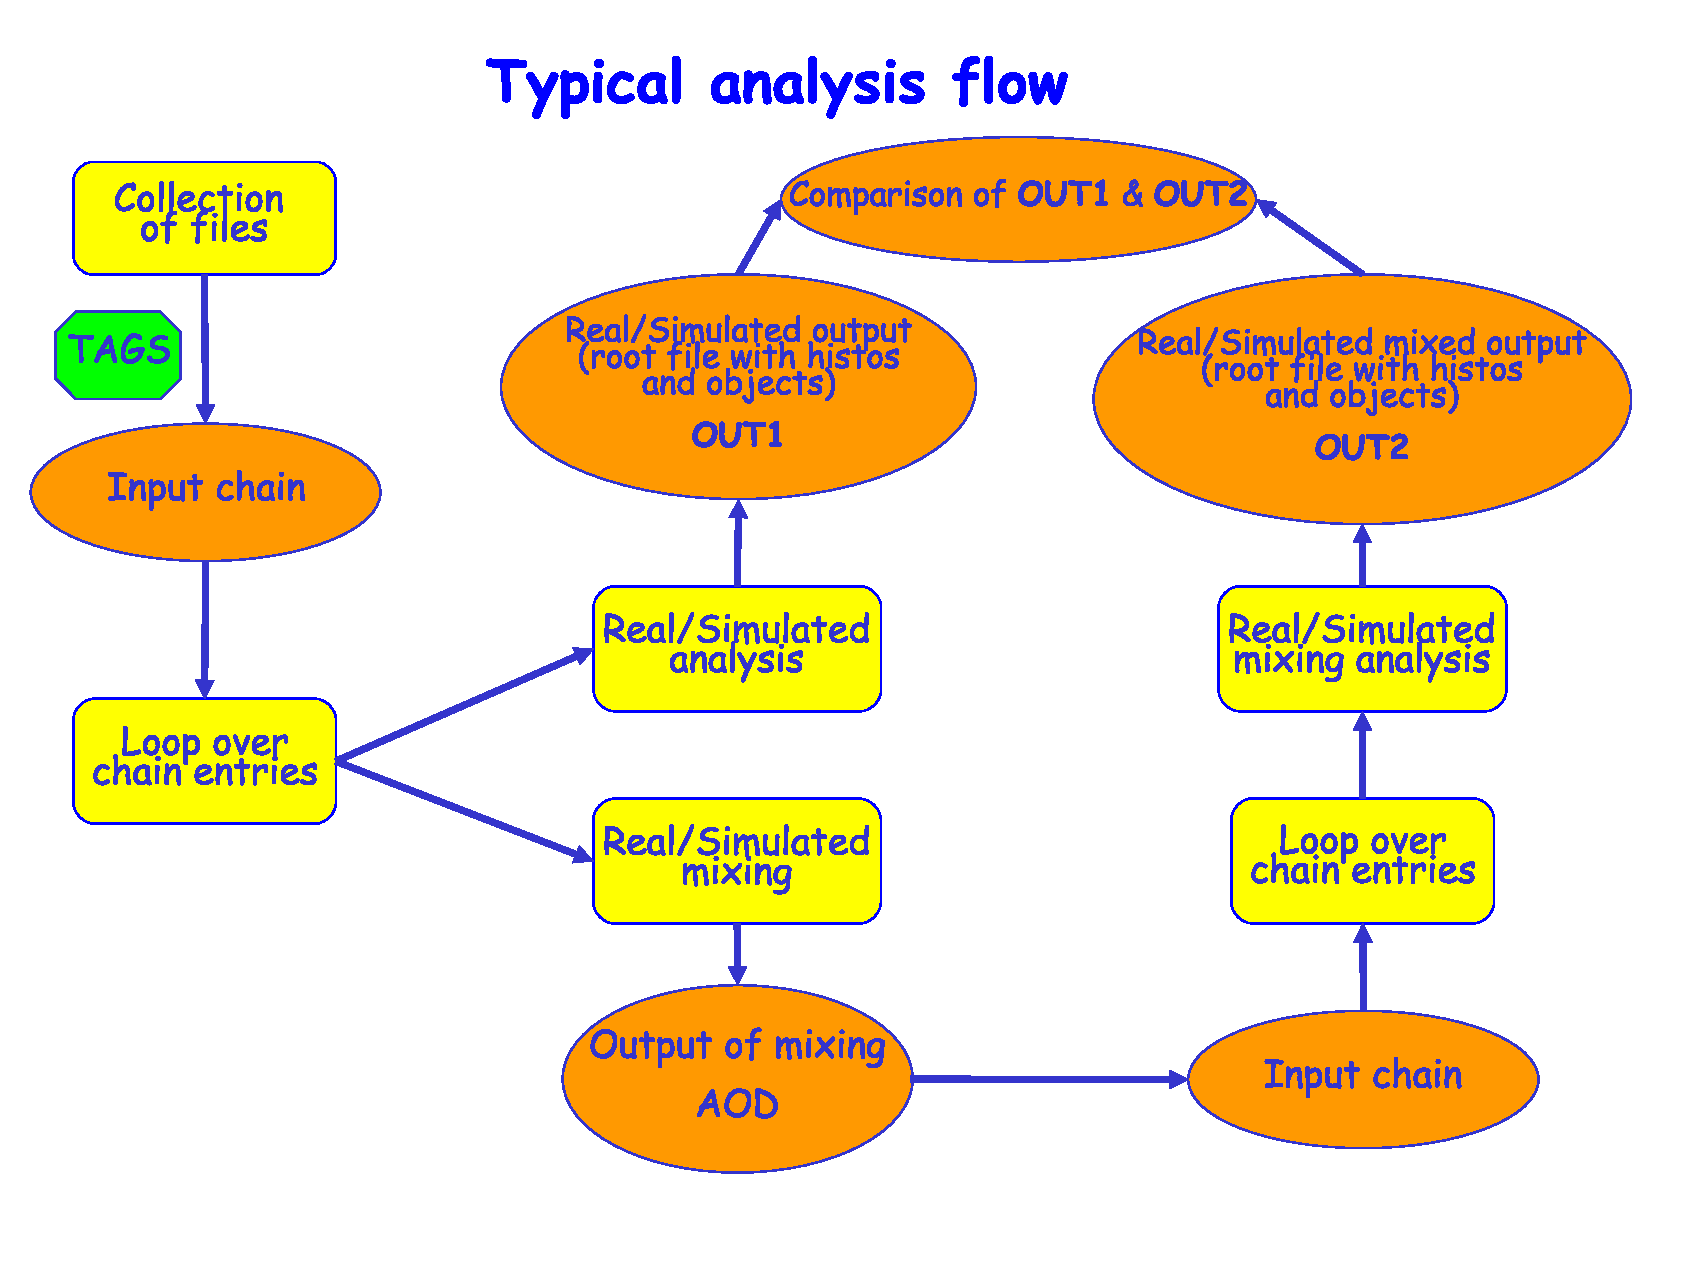
\includegraphics[width=15cm]{figures/AnalysisFramework-1.eps}
\end{center}
\caption{The flow of a typical physics analysis.}
\label{Note:FigAnalysisFramework1}
\end{figure}

\begin{figure}[ht!]
\begin{center}
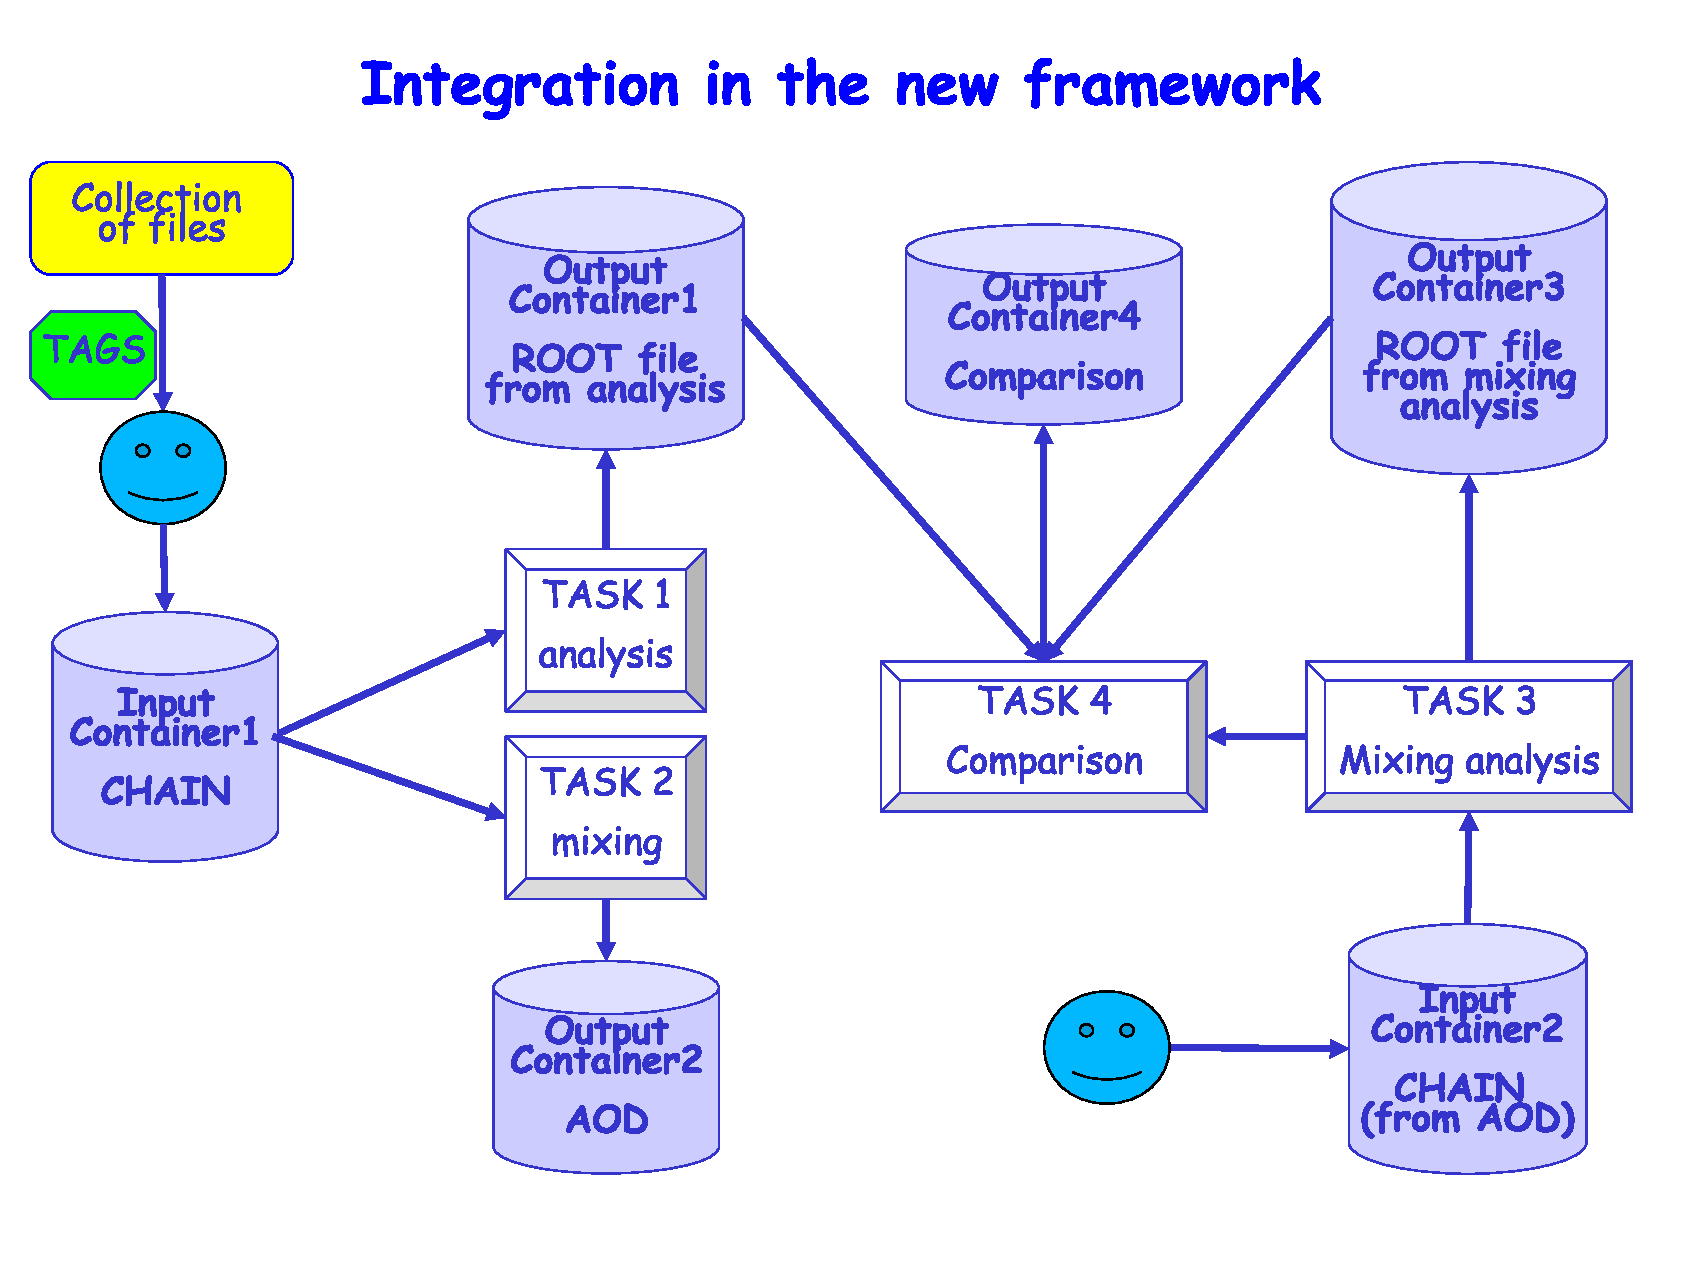
\includegraphics[width=15cm]{figures/AnalysisFramework-2.eps}
\end{center}
\caption{This figure shows how the physics analysis described in fig. \ref{Note:FigAnalysisFramework1} can be integrated in the new framework.}
\label{Note:FigAnalysisFramework2}
\end{figure}

Fig. \ref{Note:FigAnalysisFramework2} shows how we can integrate the previous use case to the new framework. The first steps are identical: A user interacts with the file catalog and creates a tag collection (as described in section \ref{Note:FLOW}) which is used as an input to query the \tag ~and create a chain of files. This chain is the first input container and is assigned to the {\ttfamily AliAnalysisManager}. In parallel we define two tasks which are also assigned to the manager and are both linked to the same input container (chain): the first analyzes the input data and creates an output container (ROOT file with histograms - signal + background plots), while the second is designed to mix the events and create a second output container (AOD). In order to analyze our mixed events, we initialize a second analysis manager which links the input container (AOD) with the new task (analysis of mixed events) and create a third output container (ROOT file with histogram - background plots). Finally the comparison task is added to the second manager. This task is triggered by the ending of the analysis of mixed events and takes two input containers (ROOT files having the signal + background plots and the pure background plots) while creating one output (extracted signal).

In the next paragraphs, we will be using the simplest possible case of manager and task which has been described in the beginning of this section.




